% ============================================================
% DIAGRAM: GPT Decoder-Only Architecture (2018)
% ============================================================
% Caption: Figure 6.2: GPT decoder-only architecture with causal masking.
%          (Adapted from Radford et al., 2018, p. 2)
% ============================================================

\documentclass[tikz,border=10pt]{standalone}
\usepackage{tikz}
\usepackage{amsmath}
\usepackage{amsfonts}

\usetikzlibrary{shapes,arrows,positioning,fit,calc,backgrounds}

\begin{document}

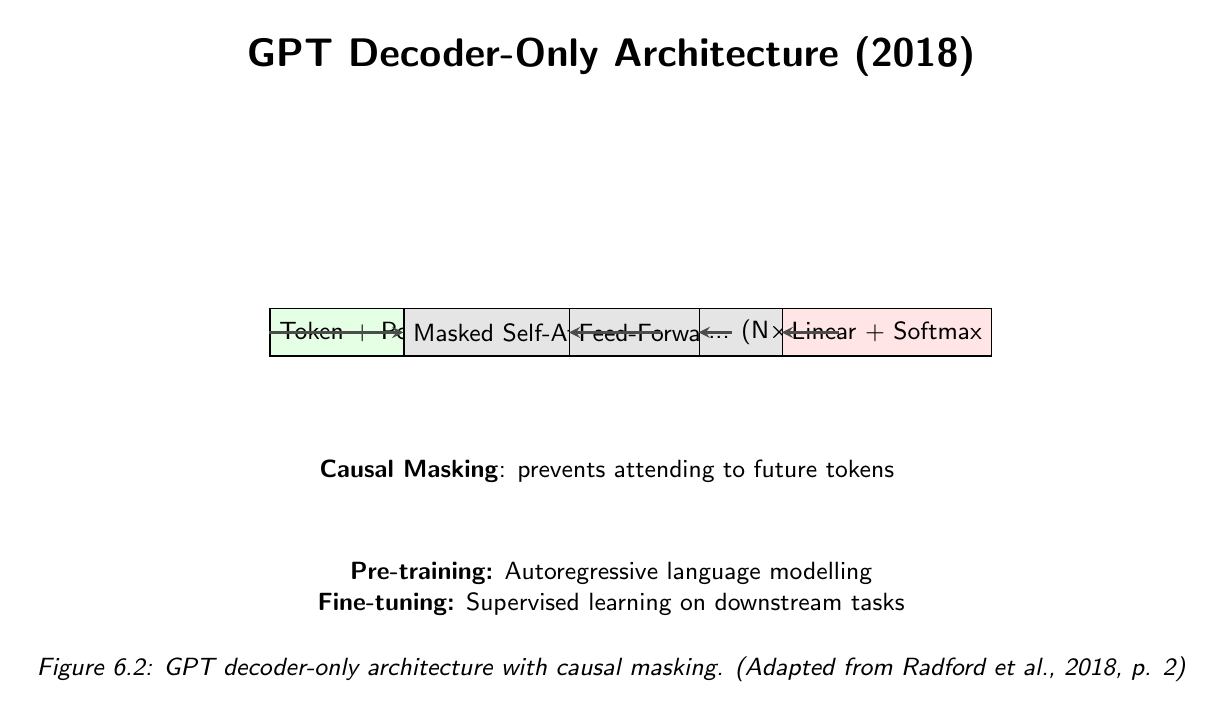
\begin{tikzpicture}[
    block/.style={draw, rectangle, minimum width=0.8cm, minimum height=0.6cm, fill=blue!10, font=\sffamily\small},
    edge/.style={-stealth, thick, draw=black!70},
    label/.style={font=\sffamily\small},
    title/.style={font=\sffamily\Large\bfseries},
    caption/.style={font=\sffamily\small\itshape},
]

\node[title] at (0, 3.5) {GPT Decoder-Only Architecture (2018)};

% Token input
\node[block, fill=green!10] (embed) at (-2.5, 0) {Token + Position Embed};

% Decoder stack (N×)
\node[block, fill=gray!20] (dec1) at (-1, 0) {Masked Self-Attention};
\node[block, fill=gray!20] (dec2) at (0.5, 0) {Feed-Forward};
\node[block, fill=gray!20] (dec3) at (2, 0) {... (N×) ...};

% Output
\node[block, fill=red!10] (out) at (3.5, 0) {Linear + Softmax};

\draw[edge] (embed) -- (dec1);
\draw[edge] (dec1) -- (dec2);
\draw[edge] (dec2) -- (dec3);
\draw[edge] (dec3) -- (out);

% Causal mask
\node[align=center, font=\sffamily\small, anchor=north] at (0, -1.5) {
  \textbf{Causal Masking}: prevents attending to future tokens
};

\node[align=center, font=\sffamily\small, anchor=north] at (0, -2.8) {
  \textbf{Pre-training:} Autoregressive language modelling \\
  \textbf{Fine-tuning:} Supervised learning on downstream tasks
};

\node[caption, anchor=north] at (0, -4.0) {
  Figure 6.2: GPT decoder-only architecture with causal masking. (Adapted from Radford et al., 2018, p. 2)
};

\end{tikzpicture}
\end{document}
